Modern IDEs provide many useful code navigation facilities, for instance
allowing users to jump from a call site to the declaration of the called
function, or to find all the call sites of a particular function definition.
The reliability of such features is contingent on the availability of accurate
call graph information. However, \matlab's dynamic typing and dynamic features
complicate the problem of statically computing a precise call graph.

Previous work on \matlab call graph construction operated on a \matlab subset,
carefully ruling out those features which aren't amenable to static analysis,
with the ultimate goal of compiling \matlab to a statically typed language such
as \fortran or \xten \cite{Tamer}. As we mean to support regular \matlab
development, carving out such a subset is not an acceptable approach.

In this chapter, we present our approach to computing an accurate call graph
for arbitrary \matlab code. Rather than relying on static analysis, we extract
this information dynamically, by instrumenting the input programs and tracing
their actual execution on a \matlab implementation. This allows us to provide
precise code navigation even in the presence of features that have
traditionally been hard to reason about statically, such as calls to
\code{eval}. This precision comes at the cost of soundness, as the computed
call graphs are correct only with respect to a set of recorded program runs,
and some extra work for the programmer, whose responsibility it becomes to
provide entry points into the project that cover enough code to be useful.

\section{\matlab features complicating static call graph computation} \label{sec:MatlabLookup}

\matlab supports a limited form of function overloading or specialization. In
particular, it has a notion of \emph{superior} and \emph{inferior} types. While
the precise rules governing this relation are not documented anywhere, Dubrau
and Hendren, after exhaustively exercising each case, produced a diagram
(reproduced in \figref{fig:BuiltinClassRelationships}) describing the superior
and inferior relationships between the different builtin types \cite{Tamer}.
This relation is not a total ordering, as, for example, a given integer type is
neither superior nor inferior to the other integer types.

\begin{figure}[htbp]
\begin{center}
\includegraphics[width=5.2in]{figures/builtinClassRelationships.eps}
\caption{Superior/inferior type relationships for \matlab. An arrow points from
$a$ to $b$ if $a$ is superior to $b$.}
\label{fig:BuiltinClassRelationships}
\end{center}
\end{figure}

When a function call is evaluated, the arguments are evaluated first, and their
types influence the function lookup. In particular, \matlab identifies the most
superior argument type -- preferring the type of the leftmost superior argument
in case there is not a unique superior type -- and uses this as the call site's
"dominant type", say \code{char}. Then, a function defined in any directory
named \code{@char/} on \matlab's path will have priority over other
user-defined functions with the same name (with the exception of functions
nested inside the call site's enclosing function). Thus, in order to statically
compute a call graph in the presence of specialized functions, we need to carry
out type inference analysis to approximate these lookup semantics.

Although \matlab's functions are not quite first-class, a special kind of
object called a function handle can be used as a reference to a function,
either named or anonymous. These handles can be stored in variables, as well as
passed and returned from functions. Thus, in order to statically compute a call
graph in the presence of function handles, interprocedural analysis is required
to track which variables might hold function handles, and also which functions
each of these might point to.

In addition to these more traditional challenges, \matlab supports many highly
dynamic features that complicate any form of static analysis. Among these are
the evaluation of arbitrary strings as code via calls to the \code{eval} family
of functions, and a function lookup mechanism that involves crawling the
filesystem at runtime -- starting from a current directory that can be changed
at runtime -- in search of applicable call targets. More attention is given to
these in \chapref{chap:DynamicFeatureElimination}.

\section{Call graph tracing instrumentation}

Since static analysis of \matlab code is difficult and easily misled in the
presence of dynamic features, we rely on dynamic analysis to extract
information that is sufficiently precise for our needs. Denker et al.
\cite{AbstractionsForDynamicAnalysis} identify different approaches available
to dynamic analysis tool developers for gathering runtime data:

\begin{itemize}
\item \emph{Source code modification} and, relatedly, \emph{logging services}.
This is the approach we ultimately use, as we discuss later.
\item \emph{Bytecode modification} or \emph{instrumenting the virtual machine}.
This requires knowledge of the internals of the \matlab virtual machine, and as
the reference \matlab implementation is a proprietary closed-source black box,
this isn't an option for us.
\item \emph{Method wrappers}. This refers to some mechanism for introducing
code to be executed before, after, or instead of a function. Our particular
source-to-source transformation, described later, can be seen of an instance of
this technique.
\item \emph{Debuggers}. While the reference \matlab implementation does include
a debugger, we prefer not to couple ourselves too tightly to it, as it is not
under our control.
\end{itemize}

The most natural and portable approach is source code modification. We can
implement it using the infrastructure provided as part of the \mclab toolkit.

The high-level idea is to insert logging statements before every possible call
site, and at the start of every function or script. After executing the
transformed code, we can post-process the logs and match up call sites with
their targets, since the target will follow the call in the log. We define a
unique identifier $identifier(n)$ for every call site and call target $n$; this
consists of the name of $n$ (the variable name if it's a variable, the function
name if it's a function definition, the script name if it's a script, and the
string \code{<lambda>} if it's an anonymous function expression), the file
it's contained in and its position (line and column) within that file. This
format comes in handy when it comes to implementing navigation features in an
IDE, as these typically take a textual range (e.g. a mouse selection) as input.

The transformation depends on a few functions (listed in
\figref{Fig:CallgraphRuntime}) being available at runtime. The
\code{mclab\_callgraph\_init} and \code{mclab\_callgraph\_log} functions
are straightforward; the former takes a path to a log file, creates it and
makes a handle to it globally accessible, while the latter takes a string and
writes it to the file. \newline \code{mclab\_callgraph\_log\_then\_run} is more
complicated; it takes a string, a variable (which is possibly a function
handle) and a variable number of arguments. If the given variable is a function
handle (either a function handle expression, or a variable that contains a
function handle), then we log the string to the file, and in either case we
forward the arguments to the variable.

\begin{figure}[htbp]
\lstinputlisting{code/callgraph_runtime.m}
\caption{The runtime components of the callgraph tracer.}
\label{Fig:CallgraphRuntime}
\end{figure}

Assuming these runtime functions are available, we traverse the whole project
and perform the following transformations.

\begin{itemize}

\item For every function or script $f$, we insert a call to
  \code{mclab\_callgraph\_log} as the first statement, passing the string
  \code{enter} followed by $identifier(f)$.

\item For every anonymous function definition $f$, we replace the body $b$ of the
  anonymous function with a call to \code{mclab\_callgraph\_log\_then\_run},
  passing the string \code{enter} followed by $identifier(f)$ as the first
  argument, and the original expression $b$ wrapped in an anonymous function
  expression taking no arguments as the second argument.

\item We replace every function call $n$ (as identified by the kind analysis)
  with a call to \code{mclab\_callgraph\_log\_then\_run}, passing the string
  \code{call} followed by $identifier(n)$ as the first argument, a handle to
  the target function as the second argument, and copies of the original
  arguments as the rest of the arguments.

  One caveat here is that there can be functions whose return value
  depends on the current execution context. For instance, \code{nargin} and
  \code{nargout} are builtin functions that return the number of input and
  output parameters passed to the current function. If we call these functions
  inside \code{mclab\_callgraph\_log\_then\_run} instead of the original
  function, they won't necessarily return the same value. As such, we avoid
  instrumenting calls to these functions, among other reflective functions such
  as \code{narginchk} and \code{inputname}. This doesn't really impact our
  precision, since these functions just return values, and can't for example
  call back into application code.

\item While the kind analysis distinguishes between function calls and variable
  accesses, it doesn't distinguish among the latter between array accesses and
  function handle invocations. In order to accurately trace control flow through
  function handles, we also instrument variable accesses in the same way as for
  function calls, only rather than passing in a function handle expression as
  the second argument, we just pass in the variable. At runtime,
  \code{mclab\_callgraph\_log\_then\_run} makes use of \matlab's reflective
  features to identify function handles, and only logs the call event in those
  cases. One small detail here is that an array access might have a colon
  literal as one of its arguments, and passing it to a function instead will
  cause \matlab to generate an error at runtime. In order for the
  transformation to be correct, we go through and replace any colon literals
  with colon string literals.

\end{itemize}

Finally, in order to trigger a tracing execution, an entry point is needed --
that is, a piece of code that will attempt to exercise as much of the subject
code as possible. This is handed off to the tracing machinery, which will first
instrument the project as described (in a temporary folder), create a temporary
file to hold the trace, and invoke \matlab, first calling
\code{mclab\_callgraph\_init} with the path to the log file, and then the
entry point. Once the execution is over, the trace is processed, and call
graph edges are identified by looking for \code{call} events that are
immediately followed by an \code{enter} event.

\figref{Fig:CallgraphBefore}, \figref{Fig:CallgraphAfter},
\figref{Fig:CallgraphTrace} and \figref{Fig:Callgraph} together show an
end-to-end example.

\begin{itemize}

\item \figref{Fig:CallgraphBefore} shows the application code.
  \code{for\_each\_file} recursively traverses a directory tree (using the
  builtin function \code{dir} as a primitive) and invokes a passed-in handler
  for each file with the given extension, making use of the helper functions
  \code{string\_ends\_with} and \code{is\_in} along the way. \code{code\_size}
  calls \code{for\_each\_file}, passing in a handle to the nested function
  \code{add\_size} as the handler. In \matlab, nested functions are closures,
  so that \code{add\_size} can read and write to the \code{total\_size}
  variable in the enclosing scope. In this way, \code{code\_size} adds up the
  sizes of all the m-files in the current directory.

\item \figref{Fig:CallgraphAfter} shows the same code after instrumentation
  (with all instances of the \code{mclab\_callgraph\_} prefix omitted for
  brevity).

\item \figref{Fig:CallgraphTrace} shows the generated trace, using an invocation
  of \code{code\_size()} as the entry point. Some events are omitted for brevity.

\item Finally, \figref{Fig:Callgraph} shows the call graph produced by
  processing the trace and matching up \code{call} and \code{enter} events.
  The call graph is in JSON format, mapping, for each covered call site, the
  call site's identifier to an array of function identifiers.

\end{itemize}

% TODO(isbadawi): Describe examples more fully.
% TODO(isbadawi): Think more about entry points. Maybe look at command history?

\begin{figure}[htbp]
\begin{minipage}{\linewidth}
  \lstinputlisting{code/callgraph-example/before/for_each_file.m}
\end{minipage}
\begin{minipage}{\linewidth}
  \lstinputlisting{code/callgraph-example/before/code_size.m}
\end{minipage}
\caption{The application code.}
\label{Fig:CallgraphBefore}
\end{figure}

\begin{figure}[htbp]
\begin{minipage}{\linewidth}
  \lstinputlisting{code/callgraph-example/after/for_each_file.m}
\end{minipage}
\begin{minipage}{\linewidth}
  \lstinputlisting{code/callgraph-example/after/code_size.m}
\end{minipage}
\caption{The same code after instrumentation.}
\label{Fig:CallgraphAfter}
\end{figure}

\begin{figure}[htbp]
\lstinputlisting[language={}]{code/callgraph-example/trace.txt}
\caption{The generated trace.}
\label{Fig:CallgraphTrace}
\end{figure}

\begin{figure}[htbp]
\lstinputlisting[language={}]{code/callgraph-example/graph.txt}
\caption{The generated call graph.}
\label{Fig:Callgraph}
\end{figure}

\section{Dealing with builtin and library functions} \label{sec:CallgraphBuiltins}

The abovementioned instrumentation can't be applied to \matlab builtin
functions. It could potentially be applied to library functions, assuming their
source code was available and they were written in \matlab and not native code.
That being said, if the goal is to enable useful code navigation features, then
instrumenting library functions is of dubious utility. In any case, during the
course of a profiling run, control flow is likely to be passed to a builtin or
otherwise uninstrumented function, which could then call back into the project
code, for instance via a passed-in function handle, a method call on a
passed-in object, or the use of \matlab's reflective features, possibly using
passed-in arguments to compute names of functions or to call. Without taking
care to handle this correctly, then in the presence of such code, our approach
will be unsound, even with respect to the recorded execution.

As an illustrative example, consider the builtin function \code{arrayfun},
which takes a function handle $f$ and an array $a$ and applies $f$ to each
element in $a$, returning an array of the outputs, analogously to the
\code{map} function in functional languages. A call to \code{arrayfun} passing
in a handle to a user-defined function $f$ will manifest in the produced call
graph as an edge linking the call to \code{arrayfun} with $f$ directly, which
isn't quite correct. That information may still be useful for code navigation
purposes, with the understanding that we're tracking how control flow jumps
through application code, rather than focusing specifically on call sites and
their targets, but there again that's beyond the scope of a call graph
computation. A bigger problem occurs if $f$ itself calls a builtin function
$c$, as control would flow back to \code{arrayfun} which would invoke $f$
again, linking together the call to $c$ with $f$. Unlike the previous case,
this has no practical application, and is just wrong.

To preserve the soundness of our approach even in such cases, we rely on more
of \matlab's reflective features. In particular, the \code{functions} builtin
function allows us to inspect the contents of a function handle at runtime, and
determine which function it points to, the path to the file in which that
function was defined if applicable, and whether or not it's a builtin function.
Using this facility, we modify \code{mclab\_callgraph\_log\_then\_run} as shown
in \figref{Fig:LogThenRunBuiltin} to insert extra markers in the call trace in
order to distinguish calls to builtin functions. These markers are ignored by
the call graph construction step, but their presence in the trace separates
builtin call sites from user-defined function entrances, avoiding the addition
of the problematic edges.

\begin{figure}[htbp]
  \lstinputlisting{code/callgraph_builtins.m}
\caption{Code to handle builtins at runtime.}
\label{Fig:LogThenRunBuiltin}
\end{figure}

% TODO(isbadawi): See "Application-only Call Graph Construction", ECOOP 2012?

\section{Instrumentation performance overhead}

A priori, we expect the instrumented code to run at least an order of magnitude
or two slower than the original code, the main culprit being the wrapping of
every single function call or variable access with a call to an auxiliary
function. In order to get a sense of the magnitude of the overhead, we run some
benchmarks with and without instrumentation. The results are shown in
\tableref{tab:InstrumentationBenchmarks}.

All the programs were executed on a machine with an Intel\textregistered \,
Core\texttrademark \, i7 CPU @ 2.4 GHz and 8 GB of memory, running OS X 10.9.4,
using \matlab version R2014b.
For each benchmark, we show the running times of the original code and the naive
instrumented version thus far. The "+ Handle prop", "- Builtins", and "+ Runtime
checks" columns are the running times with the optimizations described later in
this section. All running times are in seconds.

\begin{table}
\begin{tabular}{| l | l | l | l | l | l |}
  \hline
  Benchmark & Original & Naive & + Handle prop & - Builtins & + Runtime checks \\ \hline
  adpt        & 0.105 & 9.867    & & & 2.294\\ \hline
  arsim       & 0.259 & 0.598    & & & 0.231\\ \hline
  bbai        & 0.209 & 0.226    & & & 0.205\\ \hline
  bubble      & 0.006 & 0.010    & & & 0.010\\ \hline
  capr        & 1.068 & 1641.699 & & & 3.745\\ \hline
  clos        & 0.266 & 0.245    & & & 0.249\\ \hline
  create      & 0.033 & 0.070    & & & 0.034\\ \hline
  crni        & 1.375 & 1605.929 & & & 1.661\\ \hline
  dich        & 0.388 & 2116.571 & & & 0.394\\ \hline
  diff        & 0.140 & 243.419  & & & 0.150\\ \hline
  fdtd        & 0.117 & 0.327    & & & 0.127\\ \hline
  fft         & 0.011 & 2.138    & & & 0.019\\ \hline
  fiff        & 0.504 & 1106.703 & & & 0.506\\ \hline
  lgdr        & 0.016 & 0.024    & & & 0.019\\ \hline
  mbrt        & 0.221 & 365.613  & & & 0.993\\ \hline
  mcpi        & 0.007 & 0.013    & & & 0.011\\ \hline
  nb1d        & 1.058 & 7.209    & & & 1.076\\ \hline
  nb3d        & 0.280 & 0.616    & & & 0.311\\ \hline
  numprime    & 0.005 & 0.008    & & & 0.010\\ \hline
  optstop     & 0.014 & 0.026    & & & 0.027\\ \hline
  quadrature  & 0.003 & 0.009    & & & 0.011\\ \hline
  scra        & 0.227 & 0.262    & & & 0.253\\ \hline
  spqr        & 0.214 & 0.250    & & & 0.235\\ \hline
\end{tabular}
\caption{Running times of the instrumented code with different optimizations
enabled.}
\label{tab:InstrumentationBenchmarks}
\end{table}

\subsection{Minimizing overhead}

The bulk of the runtime overhead of our approach stems from instrumenting each
function call and variable access, which is ultimately caused by our inability
to precisely distinguish arrays from function handles statically. Yet arrays
are apt to be much more common than function handles, so that the cost of
instrumenting each array access is disproportionate relative to the benefit.
Thus, we apply a few different techniques to try and minimize the amount of
array accesses that require instrumentation.

\subsubsection{Handle propagation analysis}

While the \mclab toolkit doesn't provide any facilities for performing
interprocedural static analysis on arbitrary \matlab code, we can still track
the flow of function handles through a single function. For each use of a
variable, we can estimate whether the variable holds only data, or a function
handle, or possibly a complex data structure with a mix of data and handles.
Where we're able to determine that a variable is definitely an array containing
only data, we can avoid instrumenting it.

The \mclab framework implements such an analysis, calling it handle propagation
analysis. At each program point $p$, the analysis computes a map from
identifiers to a set of abstract values; these values are described in
\tableref{tab:HandleValues}.

To help with the definition of the analysis rules, we define two helper
functions operating on sets of abstract values. The first, $struct$, interprets
its input as representing the individual elements of an array of a cell array
$a$, and returns abstract values representing $a$ itself. The second, $sonly$,
discards from its input any values that don't represent structured data. They
are defined as follows.

% TODO(isbadawi): Rewrite above paragraph.

\begin{align*}
struct(V) &= \begin{cases}
  \lbrace DO \rbrace & \text{if } V = \lbrace DO \rbrace \\
  \lbrace DHO \rbrace & \text{if } \forall v \in V . v = H \vee v = DHO \vee v = @... \\
  \lbrace DWH \rbrace & \text{otherwise} \\
\end{cases} \\
sonly(V) &= \begin{cases}
  \lbrace DO \rbrace & \text{if } DO \in V \\
  \lbrace DHO \rbrace & \text{if } DHO \in V \\
  \lbrace DWH \rbrace & \text{if } DWH \in V \\
\end{cases} \\
\end{align*}

Given these, \tableref{tab:HandleRules} shows the rules the analysis uses to
generate abstract values for each relevant \matlab language construct. The
rules for the different kinds of expressions are largely straightforward. Of
particular interest are the last four rules, pertaining to assignment
statements. In each case, the set associated with the identifier being assigned
to is killed and replaced with the gen set.

\begin{table}
{\footnotesize
\begin{tabular}{l | l}
  \code{UNDEF (U)} & Has not been defined at this point in the program \\
  \code{DATAONLY (DO)} & Does not contain handles \\
  \code{DATAHANDLEONLY (DHO)} & Structured data, such as a struct or a cell array,
                          that only contains handles. \\
  \code{DATAWITHHANDLES (DWH)} & Structured data that can contain handles and other
                           data. This is the most general value. \\
  \code{HANDLE (H)} & Is a handle, but no information is available as to what it's
                  pointing to \\
  \code{NAMED @name} & Is a handle to a named function we know \\
  \code{ANON @(..)  ...} & Is a handle to an anonymous function we know
\end{tabular}
}
\caption{Abstract values for the handle propagation analysis.
  The \code{DO}, \code{DHO}, and \code{DWH} values are mutually exclusive.
}
\label{tab:HandleValues}
\end{table}

\begin{table}
\begin{tabular}{l | l l}
  Expression $E$ & Abstract values (i.e. $gen(E)$)  \\ \hline
  \code{@name}    & $\lbrace$ \code{@name} $\rbrace$ \\ \hline
  \code{@(..)...} & $\lbrace$ \code{@(..)...} $\rbrace$ \\ \hline

  $id$ & $in(id)$ & if $kind(id) = VAR$ \\
       & $\lbrace H, DWH \rbrace$ & if $kind(id) = FN$ \\
       & $in(id)$ & \text{if } $U \not \in in(id)$ \\
       & $\lbrace H, DWH \rbrace \cup in(id) \setminus U$ & otherwise \\ \hline

  $id(\dots)$ & $\lbrace H, DWH \rbrace$ & if $kind(id) = FN$ \\
            & $\displaystyle \bigcup_{v \in in(id)}$ of the following & otherwise \\
            & $\lbrace H, DWH \rbrace $ & if $v = H | @...$ \\
            & $\lbrace H, DWH \rbrace $ & if $v = U \wedge kind(id) \neq VAR$ \\
            & $\lbrace v \rbrace$       & otherwise \\ \hline

  $id\lbrace\dots\rbrace$ & $\lbrace DO \rbrace$ & if $DO \in in(id)$ \\
  $id.\cdots$ & $\lbrace H \rbrace$ & if $DHO \in in(id)$ \\
          & $\lbrace H, DWH \rbrace$ & if $DWH \in in(id)$ \\ \hline

  $\lbrace E_1, \dots, E_n\rbrace$ & $struct \big( \bigcup_i E_i \big)$ & \\
  $[ E_1, \dots, E_n ]$ & & \\ \hline

  any other expression & $\lbrace DO \rbrace$ & \\ \hline
  % TODO(isbadawi): Are these right?
  $id = E$ & $gen(E)$ & \\ \hline
  $id.\cdots = E$ & $sonly(in(id))) \cup struct(gen(E))$ \\ \hline
  $id\lbrace\dots\rbrace$ & $struct(in(id)) \cup struct(gen(E))$ \\ \hline
  $id(\dots) = E$ & $sonly(in(id)) \cup struct(gen(E))$ \\ \hline

\end{tabular}
\caption{Handle propagation analysis rules.}
\label{tab:HandleRules}
\end{table}

For our purposes, if the target of an array access only has the \code{DO}
abstract value associated with it, then we can safely abstain from
instrumenting it. The "+ Handle Prop" column in
\tableref{tab:InstrumentationBenchmarks} shows the performance of the
instrumented code with this enhancement applied (as a slowdown relative to
the uninstrumented code).

% TODO(isbadawi): More comments after numbers

\subsubsection{Avoiding builtin call instrumentation}

\matlab code tends to be fraught with calls to builtin functions, and
instrumenting these won't give much benefit, since we don't have access to
their source code. However, because \matlab builtin functions can be shadowed
by user-defined functions with the same name, or specialized via the mechanism
described in \secref{sec:MatlabLookup}, we can't necessarily tell statically
whether a given function call is a call to a builtin function. Because of this,
the naive instrumentation goes ahead and instruments every function call, even
if it likely is a call to a builtin.

As a conservative estimate, when we encounter a potential call to a builtin
function, we search through the project code, as well as library code, in
order to check whether any user-defined functions exist with the same name,
and only skip the instrumentation if there are no such functions. We're not
looking to statically determine the target of the call, just whether the
target might be a user-defined function. This is largely a filesystem
operation, not really static analysis. This assumes we have access to all the
code the user is apt to run, which is not an unreasonable assumption, given
that the user is the one using the static analysis.

Note that the decision not to instrument direct calls to builtins doesn't
invalidate the concerns of \secref{sec:CallgraphBuiltins}, because there
might be function handles that point to builtin functions, and in those
cases the same problem traces -- with call events that don't have a
corresponding enter event -- can arise.

The "- Builtins" column in \tableref{tab:InstrumentationBenchmarks} shows the
performance of the instrumented code with this enhancement applied.

\subsubsection{Redundant class check elimination}

Our instrumentation speculatively wraps each variable access in a function call
in case the variable is a function handle. A runtime check to determine whether
it is occurs inside this auxiliary function. This simplifies the
transformation, but is clearly wasteful if the variable turns out to be a plain
array variable, especially if the variable is accessed more than once. Since
\matlab is used a lot for numerical computations, \matlab code tends to be
heavy on loops, such that array variables are often accessed repeatedly,
magnifying the overhead. Intuitively, we should be able to check the type of a
given variable only once, and avoid instrumenting accesses to it at all if it's
not a function handle.

However, this presents a complication in terms of implementation complexity.
Wrapping each variable access in a function call is a very simple
transformation to make, as it just involves replacing an expression AST node
with another. If we start introducing conditionals, the transformation becomes
a lot more intrusive, since \matlab does not support any kind of conditional
expression (such as the ternary \code{\?:} operator in C-based languages), only
conditional statements. Thus, inserting checks at the right places while
preserving the order of operations requires destructuring the code into a kind
of three-address form.

The handle propagation analysis is precise enough in practice if we restrict
ourselves to a single function -- a lot of the imprecision occurs when arrays
are passed around as function parameters. As a simple middle ground, we insert
a single runtime check at the start of each function, checking whether any of
the arguments to the function is a function handle. In the then branch, we
insert the original instrumented version of the function. In the else branch,
we insert another copy of the function where we avoid instrumenting any uses of
the function parameters. A still more sophisticated approach would be to run
the handle propagation analysis once for each version with different initial
information.

\section{Minimizing call graph invalidation}

The call graph computed from a profiling run maps source positions to other
source positions. As such, it is extremely sensitive to even minor changes to
the project code -- even ostensibly inconsequential changes like adding
whitespace or comments would invalidate portions of the call graph as tokens
are shifted around. A sufficiently sophisticated implementation can ward
against this by keeping track of the moving tokens and computing offsets as
needed before querying the call graph. A larger issue is that, a priori, the
effect of a textual code change on the call graph is not obvious, requiring us
to update the call graph in the face of any change, no matter how minor, in
order to ensure stale edges are excised. Further, profiling doesn't really lend
itself to any sort of incremental call graph updating scheme; our only real
means of updating the call graph is to invalidate it and replace it with the
result of triggering another execution. Depending on the project and the
provided entry point code, each execution could potentially be expensive --
likely too expensive for our purposes, since in an IDE, unlike in some other
applications of call graphs, the code is apt to be in constant flux,
practically requiring us to be triggering an execution whenever the user stops
typing. Given all this, we would like to somehow make our call graph more
robust in the face of code changes.

\subsection{Multiple entry points}

Rather than relying on a single entry point to guide profiling runs, multiple
entry points can be provided, ideally each small and independent, analogously
to different tests in a unit test suite. During the profiling run, each entry
point is executed in turn, each resulting in its own call graph. These are then
combined into a composite call graph, queries against which are resolved by
forwarding them to each component call graph in turn and concatenating the
results together.

The advantage of this approach is that each entry point's call graph can be
invalidated independently. When a file is modified, only call graphs where at
least one node corresponds to a position within that file are discarded. When
queries are submitted to the composite call graph, it can attempt to answer
them with the remaining information. A profiling run only needs to be triggered
if the query comes up empty, and only the invalidated entry points need to be
executed again.

% TODO(isbadawi): Does this make sense? Because call graph queries can have
% multiple answers, so even if your result is nonempty, updating the call
% graph could still give you more.

\subsection{Classifying edits}

Rather than invalidating the call graph on every change, we can try to be more
discriminating. As alluded to earlier, it is likely difficult if not impossible
in general to reliably predict whether a given change requires an update to the
call graph. However, given a description of the differences between the two
versions of the code, we can apply some heuristics to avoid recomputation in
some cases. If we can somehow determine that a given change will have no effect
on the call graph, then we just need to keep track of offsets to add to token
positions before querying the call graph.

A natural first approach is to parse both versions of the code and apply a tree
differencing algorithm on the two ASTs. If the trees have the same structure,
which might happen if the change affected only the layout of the code, for
instance by adding or removing comments or adjusting the indentation, then the
behavior of the code is the same. Parsing might be expensive, but is likely to
be required by different components of an IDE anyhow; for example, a typical
feature provided by IDEs is syntax checking, whereby syntax errors are
presented to the user as they type. Thus, there is only the added cost of
applying the differencing algorithm.

% TODO(isbadawi): Flesh this out, more formal

% Maybe parsing is not required in some cases -- can determine whether a
% change is whitespace only just by looking at the diff.
% (but MATLAB is whitespace sensitive in some cases...)
% But if we're parsing anyway, does this matter?

\section{Related work}

% Look at trace summarization, or compaction?

% Look into context-sensitive call graphs? Would be neat, but not sure what
% a good UI would be to exploit this information in the IDE...

% "Efficient Construction of Approximate Call Graphs for JavaScript IDE Services", ICSE 2013
